% multipath execution on a large distributed microarchitecture
%
%\documentclass[10pt,twocolumn,dvips]{article}
\documentclass[10pt,dvips]{article}
\usepackage[english]{babel}
\usepackage{epsfig}
%
%\usepackage{fancyheadings}
%\usepackage[T1]{fontenc}
%\usepackage[latin1]{inputenc}
%
%\usepackage{twocolumn}
%\usepackage{verbatim,moreverb,doublespace}
%\usepackage{rotate,lscape,dcolumn,array,rotating,latexsym}
%
%\input{epsf}
%
\textwidth 6.5in
\textheight 9.0in
\topmargin -0.6in
\oddsidemargin 0mm
\evensidemargin 0mm
%
\pagestyle{empty}
%
\begin{document}
\parskip 3mm
%
%
\title{Mutlipath Execution on a Large-Scale Distributed 
Microarchitecture}
%
\author{
A. Khalafi, D. Morano, D.R. kaeli\\
Northeastern University\\
{kaeli, akhalafi, dmorano}@ece.neu.edu\\
\and
A.K. Uht \\
University of Rhode Island\\ uht@ele.uri.edu
}
%
\maketitle
\thispagestyle{empty}
%
\begin{abstract}
This paper explores the implementation of multipath execution on a
large distributed microarchitecture.  With the advent of the
possibility of large microarchitures, means to mitigate, or help to
mitigate, the deleterious effects of branch mispredictions need to be
more aggressively explored.  We suggest that multipath execution is one
way to approach the continuing problem of branch misprediction
penalties.  Further, with a microarchitecture that now allows for very
large numbers of instrcutions to be simultaneously in the process of
being executed, multipath execution provides a more efficient use of
hardware execution resources than continuing to speculatively execute
hundreds or more instructions down a single path.

We briefly present the outline of a large scale distributed microarchitecture
and discuss how we overlay multipath execution on it.
We provide simulation results for several microarchitectural configurations
that demonstrate the positive effects of multipath execution in
hiding and mitigating the inevitable branch mispredictions.
\end{abstract}
%
\section{Introduction}
%
Performance penalties due to mispredicted branches continue to
present a challenge for achieving higher performance execution
of single threaded programs.
These penalties restrict the instruction level parallelism (ILP)
that might be achieved if they could be mitigated.
One approach towards reducing the negative effects of mispredicted
branches, and a moderately successful one, has been the pursuit
of better branch predictors.  However, many branches in typical
programs remain difficult to predict accurately and these continue
to limit performance in many codes.

Another approach towards mitigating the effects of mispredicted branches
has been that of attempting to address the problem of executing
down both paths of a branch in some measure or another before the
branch is able to resolve.  This approach is not new but presents
complexity problems that have made it less than attractive for
many practical processor designs.  However, with the advent of ever
increasing amounts of speculative execution, the need to address
the problems associated with mispredicted branches has only grown worse.

Current commercial machines have only as yet been designed for modest
amounts of speculative execution (usually several instructions to 
less than about 40 instructions per thread).
However, for applications which demand it,
future machines may need to execute upwards of one hundred to
several hundreds of instructions speculatively in order to maximize
performance.  This trend will only increase the pressure to try
and reduce the effects of branch mispredictions than we tolerate
at present.

Our work presented in this paper is oriented towards reducing the
negative effects of mispredicted branches through multi-path execution
while doing so on an aggressive large-scale (able to speculatively execute
possibly hundreds of instructions simultaneously)
distributed
microarchitecture.  The large distributed microarchitecture offers the
possibility to significantly step up programs speedups through ILP.
However, many problems common to more conventional processor designs
are either at least as difficult to deal with on a large-scale
microarchitecture or indeed become more difficult to deal with.
The problem of mispredicted branches is one of these latter problems.
The penalty associated with a mispredicted branch can now means
the possible squashing and associated opportunity lost of possibly
hundreds of instructions that were in flight.  Clearly this
is not the most desirable consequence to be resigned to accept.

Another issue that arises in large-scale microarchitectures is the
problem of efficient execution resource usage.
As we may speculatively execute many branch paths ahead of execution
commitment along the most predicted path in the program, the likelihood
of the newest (latest) most speculatively executed instruction to
be committed (part of the program's committed execution trace) tends
towards zero.  At a certain point, the likelihood of the committed (correct)
program execution to proceed down an alternative program path
besides the one defined by each sequential predicted branch outcome
becomes greater.  This would indicate that for very large speculative
machines, multi-path execution is all but a necessity to most
efficiently allocate and use the available execution resources.

Our present work on multipath execution is part of a larger
desire to explore large-scale ILP speedups in sequential programs.
This goal has been motivated through the work of researchers like
Lam and Wilson
~\cite{Lam92},
A. Uht and V. Sindagi ~\cite{Uht95},
J. Gonzalez and A. Gonzalez ~\cite{Gon97}.
In this paper, we briefly present an overview of our large-scale distributed
microarchitecture suited for achieving large ILP speedups.  
We then propose a strategy for handling
multipath execution on this microarchitecture.

The rest of this paper is organized as follows.
Section two provides some background on multipath execution.
Section three presents an overview of our large-scale distributed
microarchitecture.
In section four, we provide some analysis of the conditional
branches in some benchmark programs.  We will also discuss how we
would like to 
spawn speculative execution paths
in response to certain conditional branches of each category that 
are encountered.
Section five presents some simulation results for various
configurations of our machine and how multipath execution
changes the results when applied.  Shown first are simulation
results for various machine configurations when execution in
Single Path (SP) mode only.  We then show results for
the same benchmark suite with varying numbers of additional
speculative execution paths.
And we summarize and conclude in section seven.
%
\section{Background on Multipath Execution}
%
Attempts at performing some form of multipath execution 
are quite old now.  Early work was dominated by IBM in the
late 1970s and 1980s \cite{Conners79}.
The earliest attempts at multipath
execution started with the ability to prefetch down both
paths of a conditional branch.  This became more aggressive
to the point of actually executing down both outcomes of
a conditional branch.  Aggressively executing down both outcomes
of conditional branches has been explored in the work
by S.S.H Wang \cite{Wang90}.  
More aggressive research by Uht and
Sindagi \cite{Uht95} explored the intersection of both
multipath execution and future large-scale microarchitectures
capable of possibly hundreds of instructions being executed simultaneously.
They also addressed the general question of speculatively executing
more than two paths simultaneously.
Work on dual path execution (only two speculative paths) has
been done by Heil and Smith \cite{Heil96}.
Examining multipath execution on the PolyPath microarchitecture,
Klauser et al explored several implementation details
as well as demonstrating an improvement of three speculative paths
over just having two.

An increasingly attractive approach to multipath execution is that
of using a basic simultaneous multi-threaded (SMT) processor
to provide the resources for essentially executing multiple paths
of a single architected program thread.  This work follows from
the original SMT idea and followed from the work by
Tullsen et al \cite{Tullsen96}.  The work by Tullsen et al focused
on making better use of the processor when
branch mispredictions are encountered by filling processor resources with
work from other architected threads following a misprediction.
An extension of this idea is to use resources for executing
the alternative path (not predicted path) of a mispredicted branch.
An example of this approach has been discussed by 
Wallace et al \cite{Wallace98}.  This general approach of combining
both simultaneous multithreading with multipath execution appears
to be good compromise to the problem of most efficiently using
processor resources for a possibly programmable desired work load
characterization (best single architected thread performance or
best overall processor multithread throughput).  Other efforts
appear to be focusing on these sorts of SMT tradeoffs and
it appears that, although apparently not pursuing multipath execution, 
Sun Microsystems
is planning for some dynamic processor customization along these lines 
with the Ultra-SPARC IV processor.

Ahuja et al \cite{Ahuja98} explore some limits for speedups from
multipath execution but their work is still largely restricted to more
conventional (modest sized) microarchitectures with less than 128
speculative instructions in flight.  Our present work explores the use
of multipath execution on a significantly larger microarchitecture than
that of Ahuja or the other past work with the exception of that by
Uht and 
Sindagi \cite{Uht95}.
Our present work is capable of having several hundred or more
speculative instructions in flight and is most patterned after the
work by Uht.
%
\section{A Large-scale Distributed Microarchitecture}
%
Our primary goal is to converge on a microarchitecture suitable
for extracting large ILP speedups from sequential programs.
This has resulted so far in a very aggressive large (and scalable)
microarchitecture capable of having many hundreds or perhaps thousands
of speculatively executed instructions in flight.  Scalability
of the microarchitecture is achieved through its distributed nature.
In general, scalability requires little to no dependence on major
central microarchitectural hardware structures in the machine.
This goal presents many challenges (not further enumerated here)
to say the least but the efficient handling of multipath execution
is one of those challenges.  A brief overview of our general
large-scale distributed microarchitecture is presented in the following
sections.
%
\subsection{Basic Microarchitecture Components and Layout}
%
An overall high-level view of the core of our microarchitecture is shown in 
Figure \ref{fig:window}.

\begin{figure}
\vspace{0.2 in}
\setlength{\epsfxsize}{10cm}%7
\centerline{\epsfbox{window.eps}}
%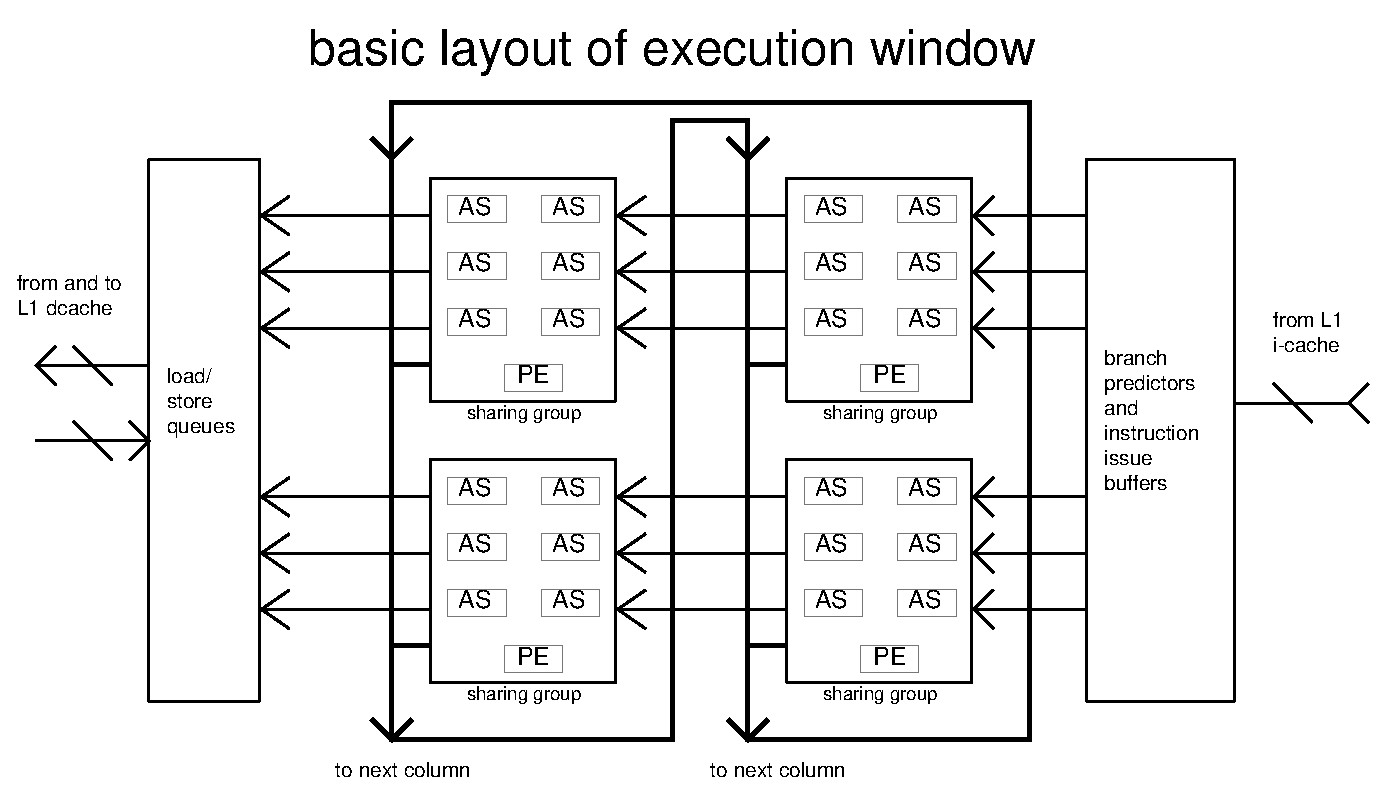
\epsfig{file=window.eps,width=5.8in}
\caption{{\em High-level View of the Distributed Microarchitecture.} 
Shown is a layout of the Active Stations and Processing Elements
along with some bus interconnections to implement a large,
distributed microarchitecture.}
\label{fig:window}
\end{figure}

We have extended the idea of Tomasulo's reservation
station \cite{Tom67} to provide the basic building block for a distributed
microarchitecture.  Tomasulo's reservation station provided for the
simultaneous execution of different instructions over several
functional units.  This part of his scheme (already widely used) is
retained but extended to forward execution results to other spatially
separated and distributed reservation stations and execution units
rather than looping the results back to a common instruction issue unit
and update logic for the architected register file.  We also extend the idea
of the reservation station to allow for multiple executions (re-executions)
of the same instruction in the station.  We keep 
instructions in their associated stations station until they are retired 
(either committed or 
squashed).  
We call our adaptation of the reservation station the
\textit{active station}, abbreviated \textit{AS}.  

Rather than lay the active stations out in silicon simply next to
function units that will execute the instructions issued to them
(like with the original reservation station idea),
we lay them out in a two dimensional grid whereby sequentially
issued instructions will go to sequential ASes down a column of
the two dimensional grid of ASes. 

Dispersed among the active stations are associated execution
units.  These executions units are represented in the figure as
a \textit{processing element}, abbreviated \textit{PE}.  
Although an AS always only holds at most a single instruction,
PEs may consist of a unified all-purpose execution unit capable of
executing any of the possible machine instructions or
several functionally partitioned units individually tailored
for specific classes of instructions (integer ALU, FP, or other).

Groups of active stations along with their associated processing
element
are termed \textit{sharing groups}.  Sharing groups somewhat resemble
the relationship between the register file, reorder buffer,
reservation stations, and function units of most conventional
microarchitectures.  They have a relatively high degree of bus
interconnectivity between them as conventional microarchitectures do.
In our case, the active stations serve the role of both the
reservation station and the reorder buffer of more conventional
machines.

A scalable interconnect fabric 
is provided to forward result
operands from earlier active stations to latter active stations in
program order.  Result operands consist of register, memory, and
instruction predicates.  We also employ a strategy of predicating all
issued instructions within the microarchitecture itself.  This is also 
invisible from the instruction set architecture of the machine.
The interconnect fabric is simply shown by
the bold vertical buses in the figure.  These result-forwarding buses
loop around from the bottom of left adjoining columns to the tops of
the right adjoining columns.  The forwarding from the far lower right
also loops around to the far upper left.  In all, the forwarding
buses (interconnection fabric) form the characteristic ring pattern
passing by each sharing group in the execution window.
It should be noted that the interconnection fabric is not
entirely passive (or else the microarchitecture would not
scale to large sized) but rather is an active network.
Several active networks are possible.  We used a simple one
in the present work where a group of four parallel buses transport
result operands to subsequent sharing groups.  The buses are repeated
at a fixed interval of every four sharing groups.

The less bold horizontal buses
form the paths by which instructions are issued to active stations
from the decoded instructions buffers, shown on the far right.
Variations in instruction buffers are possible and may be thought
to resemble trace caches or a sort.
Finally, on the far left, horizontal buses take committed program
stores from retired store instructions residing in the active stations
to the load/store queues (one per row).
The two dimensional
grid of active stations along with their interspersed processing elements
is termed the \textit{execution window}.

Figure \ref{fig:window}, as an example machine configuration, consists of 
two columns of sharing groups.  Each sharing group contains two columns of
active stations (the specific use of which is explained later).
Each sharing group also contains three rows of active stations
and a single processing element in the shown case.  
We generally characterize
a basic machine configuration according to the triple: sharing group
rows, active station
rows per sharing group, and sharing group columns.  We normally
show these numbers concatenated with a hyphen so the machine shown
in the figure would be abbreviated {\tt 2-3-2}.

The instruction fetch unit (not shown) is responsible for
fetching instructions from the memory hierarchy, these are then decoded
and placed into the issue buffers.   
Currently, branch predictors are provided one per AS row of the execution
window.  
They are located between the issue buffers and the buses that feed
decoded instruction information into the execution window and the
active stations.  The branch predictors are queried for both
a prediction of the branch outcome as well as a confidence
indication of that prediction.  This information flows along with
the decoded instruction itself into the
execution window when insstructions are issued to the active stations.
Updates of the branch predictors come from resolved branches
of the same row that they each serve.

Not shown in the Figure, and outside of the execution window,
lies address interleaved L1 instruction and data caches, along with
interleaved L2 I/D caches and finally, interleaved main memory.
Interleaving of the entire memory subsystem is generally necessary
to provide sufficient bandwidth for instruction fetching and the
enhanced load bandwidth needed for large sized machines.

Our microarchitecture is roughly characterized as a Control Dependence
based Decentralization (CDD) as termed by N. Ranganathan and
M. Franklin~\cite{Ranganathan98}.
Although execution in this microarchitecture is not strictly
characterized by control dependence but rather primarily by
general data dependence (including control converted to data),
the grouping of execution resources roughly follows a control
oriented graph of the program thus best characterizing it as above.
%
\subsection{Basic Machine Operation}
%
Instructions are fetched from memory, decoded, and staged in buffers
(not too dissimilar from trace caches).  Variation in fetch buffer
design has been considered but it is not discussed in more detail here.
When an entire column
of active stations is free to accept new instructions, generally
an entire column of instructions are issued to the free active station
column from a fetch buffer.
Conditional branches are
predicted at or just before instructions issue to the ASes.
Both a prediction of the branch outcome as well as an indication
of the confidence of the prediction is sent along with the
decoded instruction information when instructions are issued to
ASes.

All of the active stations in a given column are issued instructions
in a single clock.  Currently, if a column is issued instructions
and some
active stations in that column had no associated or meaningful
instruction waiting to issue to them, then those ASes are marked
as being unused in that column.  This is a source of reduced IPC but, as will
be explained later, other sources of wasted or inefficient use of
active station resources are also possible.
In our present implementation, newly issued instructions
are only issued to a single column of active stations within
a solumn of sharing groups.  The other column of active stations
in our current sharing groups (which currently have a total
of two columns of ASes) is reserved for the spawning of additional
execution paths as a result of a condition branch instruction.
When and how additional paths are spawned is discussed later.

It should be noted that there are several strategies for
issuing instructions to available active station columns.
Since all issued instructions are speculative, instructions
from either outgoing path of a conditional branch can be issued
to sequential active stations.
The fetch unit is responsible for preparing for such decisions.
Even when a conditional branch is predicted as being taken,
instructions may still be issued sequentially down the not-taken
path under certain circumstances.  If the distance to the target 
of a branch
that is predicted to be taken is not too large,
instructions may be issued along the program static order (or not-taken
path) of the branch in the hopes of capturing hammock styled branch
constructs.  A more detailed dicussion on these alternatives is
presented later in the paper.

Program dependencies (control, register, and memory) are 
maintained through the use of tags that
are associated with all forwarded operands.
This has some resemblance to register tags used in more conventional 
microarchitectures but has been more generalized for use in this
distributed microarchitecture.  Instructions remain in their
associated active stations until they are retired by either being
committed or abandoned (squashed).  In this way, the active stations
(or rather the whole set of them)
fulfill the role of the reorder buffer or register update unit of more
conventional microarchitectures.
The exact details of the enforcement of program dependencies
is not covered further in this paper.

Much more detailed information about this microarchitecture
can be found in a technical report by Uht et al~\cite{Uht01}.
Additionally, a more detailed discussion of the mechanism used for
enforcing program dependencies in this microarchitecture
can be found in a report by Kaeli et al~\cite{Uht01}.
A more detailed discussion about mutipath spawning is given
in the following section.
%
\section{Conditional Branch Characterization and Handling}
%
In this section we provide a short analysis of the conditional
branches are are found in the suite of benchmark programs that
we are investigating.  We will follow this up with how we would
like our machine to react to encountering the different types of
branches encountered.  Essentially, machine decisions about
spawning second and subsequent speculative execution paths is governed
in part by the types of conditional branches encountered.
%
\subsection{Conditional Branch Characterization}
%
Since the good handling of conditional branches is important
in any microarchitecture that spawns additional speculative
paths for unresolved branches, some attention is given
towards characterizing their behavior.  We focused
on five benchmark programs for characterizing branch behavior.
The benchmark programs explored along with some statistics on each
are :

\begin{tabular}{|c|c|c|c|}
\hline 
benchmark&
br. pred. accuaracy&
avg. L1 miss rate&
dynamic cond. braches\\
\hline
\hline 
go&
72.1\%&
96.6\%&
9.0\%\\
\hline 
gap&
94.5\%&
98.9\%&
6.2\%\\
\hline 
parser&
92.6\%&
98.3\%&
13\%\\
\hline 
gzip&
85.4\%&
97.0\%&
8.8\%\\
\hline 
bzip&
90.5\%&
98.5\%&
7.0\%\\
\hline
\end{tabular}

The 
{\tt go} benchmark is from the SpecInt-95 suite while the rest
are from the SpecInt-2000 suite.

Since our microarchitecture is suited towards especially handling
hammock styled conditional branch constructs, we were interested
in the size of the branch domains for both all branches
dynamically executed in the programs as well as for those branches 
that contribute most to mispredictions.
Figure \ref{fig:numbranches} shows a probability distribution of
the percentage of the number of dynamic branches that occur at
or below a branch domain size.  

\begin{figure}
\vspace{0.2 in}
\setlength{\epsfxsize}{10cm}%7
\centerline{\epsfbox{numbranches.eps}}
%\centering
%\epsfig{file=numbranches.eps,width=5.8in}
\caption{{\em Probability Distribution For Dynamic Branches for 
Branch Domain Size.} 
Shown are the percentage of dynamic branches versus branch domain size
in instructions.}
\label{fig:numbranches}
\end{figure}

Figure \ref{fig:mispredictions} shows a probability distribution of
the percentage of the number of branch mispredictions that
occur for branches at or below a branch domain size.
From these two figures it can be seen 
that a large fraction of total misses is due to branches with small domain
size. 

\begin{figure}
\vspace{0.2 in}
\setlength{\epsfxsize}{10cm}%7
\centerline{\epsfbox{mispredictions.eps}}
%\centering
%\epsfig{file=mispredictions.eps,width=5.8in}
\caption{{\em Probability Distribution For Branches Mispredictions
versus
Branch Domain Size.} 
Shown are the percentage of dynamic branch mispredictions versus 
branch domain size
in instructions.}
\label{fig:mispredictions}
\end{figure}

To get a better understanding of how to handle differnt branches,
we proceeded to define four orthogonal characteristics
for conditional branches that might give us insight into
how they might be handled in the microarchiteture.
This creates a total of sixteen classes into which all conditional 
branches are placed.
The four characteristics used to classify each conditional branch are :

\begin{itemize}
\item{execution frequency}
\item{branch predictability}
\item{direction of the branch target -- forward or backward}
\item{distance to the target of the branch}
\end{itemize}   

We classify each conditional branch as 
being either a high dynamic frequency branch
or a low dynamic frequency branch.  If the conditional branch
is within the top 90\% of all dynamically executed conditional branches,
it is classified as a \textit{high} frequency branch, else it 
is \textit{low} frequency.
For each conditional branch, we accummulate statistics on
its predictability.  If the branch is 95\% or more predictable
it is assumed to be 
\textit{predictable}, else we assume that it is
\textit{unpredictable}.
The direction of the branch is also recorded and is simply
refered to as being either a 
\textit{forward} branch or a 
\textit{backward} branch.
Finally, the distance of the branch to 
the instruction at the
branch targer is computed and recorded.  The distance is measured
in instructions.  If the target of the branch is less than 170 instructions
from the branch itself, the branch is considered to have a 
\textit{near} target, else it is considered to have a
\textit{far} target.  The value of 170 instructions was chosen
because for many of the machine configurations that we will be
investigating, this number is approximately between one half of
the possible number of speculatively executed insturctions
that can be inflight and two thirds of the total possible number.
This will be clarified later.

Using the above numbers, we calculate the percentage of branches that fall into each category.  Table xxxx shows the statistics for each benchmark.  



In the next section, we discuss how we would like to try and
use the available machine run-time information on branches to
govern how best to spawn additional speculative execution paths
in response to specific conditional branches encountered during execution.
%
\subsection{Machine Handling of Conditional Branches}
%
The run-time machine microarchitecture only has limited information
available to it for making certain optional decisions.
There are two major alternatives that the machine needs to constantly
consider.  The first is whether to issue instructions to sequential
ASes following
the not-taken path of the condition branch or to issue instructions
along the 
taken path.  The second decision to make is
whether to spawn an alternative speculative path
on any given conditional branch.
Basically, the machine only has the following information
available at run-time for making microarchitectural decisions :

\begin{itemize}
\item{branch prediction confidence}
\item{distance to the target of the branch}
\item{branch target direction -- forward/backward}
\item{the branch outcome prediction}
\end{itemize}   

For most of the branches with small domain size, static fetch will
provide the benefit of having both the domain and target of the branch 
in the instruction window.  This is an important factor for reducing
branch penalties without having a complex fetch unit.  On the other
hand, for the branches with distant target that have a hight 
probility of being taken, this approach might result in poor performance.
In our architecture, if a branch has a far target and it is highly predicted
to be taken, we choose to continue fetching from the target of the branch.

%
\section{Simulation Results}
%
We present results from simulations of a set of machine configurations
using the general microarchitecture described.
%
\subsection{Methodology}
%
The simulator is a recently built tool that shares some similarity
to SimpleScalar \cite{Austin97} but which was not based on it.
We execute
SpecInt-2000 and SpecInt-95 programs on simulated machines
that feature a MIPS-1 ISA along with the addition of some MIPS-2 and
MIPS-3 ISA instructions.  We are using the standard SGI Irix system
libraries so we needed some MIPS-2 and MIPS-3 instructions to accommodate
that.  All programs were compiled on an SGI machine under Irix 6.4 and
using the standard SGI compiler and linker.  The code was compiled with
standard optimization ({\tt -O}) for primarily the MIPS-1 ISA ({\tt -o32}).
%
\subsection{IPC Results and Discussion}
%
The data below are IPC results for various sized configurations of
a machine.  The general features of
the machine simulated are 100\% hit rates for L1 instruction cache,
a 1 cycle hit delay and 20 cycle miss penalty for the L1 data cache,
100\% hit in the L2 data cache, an operand forwarding delay of 1 clock
and a general bus delay of 1 clock.  The data cache is 32kB 2-way
set associative that is also 4-way interleaved on address bits 2 and 3.

Presented in 
Figure \ref{fig:ipc} are IPC results for each of the benchmark
programs over various machine configurations.
The results of each benchmark program for varying machine
configurations is given each group.  The benchmarks are from left to
right in the figure: 1) {\tt go}, 2) {\tt gap}, 3) {\tt bzip2},
4) {\tt gzip}, 5) {\tt parser}.  Each group of results respresents
the IPC rsulting from each of the following machine configurations (left
to right) :

\begin{tabular}{|c|c|c|}
\hline 
SG rows&
ASes per SG&
SG columns\\
\hline
\hline 
8&
4&
16\\
\hline 
8&
4&
8\\
\hline 
8&
8&
8\\
\hline 
8&
8&
16\\
\hline 
8&
16&
16\\
\hline 
8&
16&
8\\
\hline
\end{tabular}

\begin{figure}
\vspace{0.2 in}
\setlength{\epsfxsize}{10cm}%7
\centerline{\epsfbox{ics1.eps}}
%\centering
%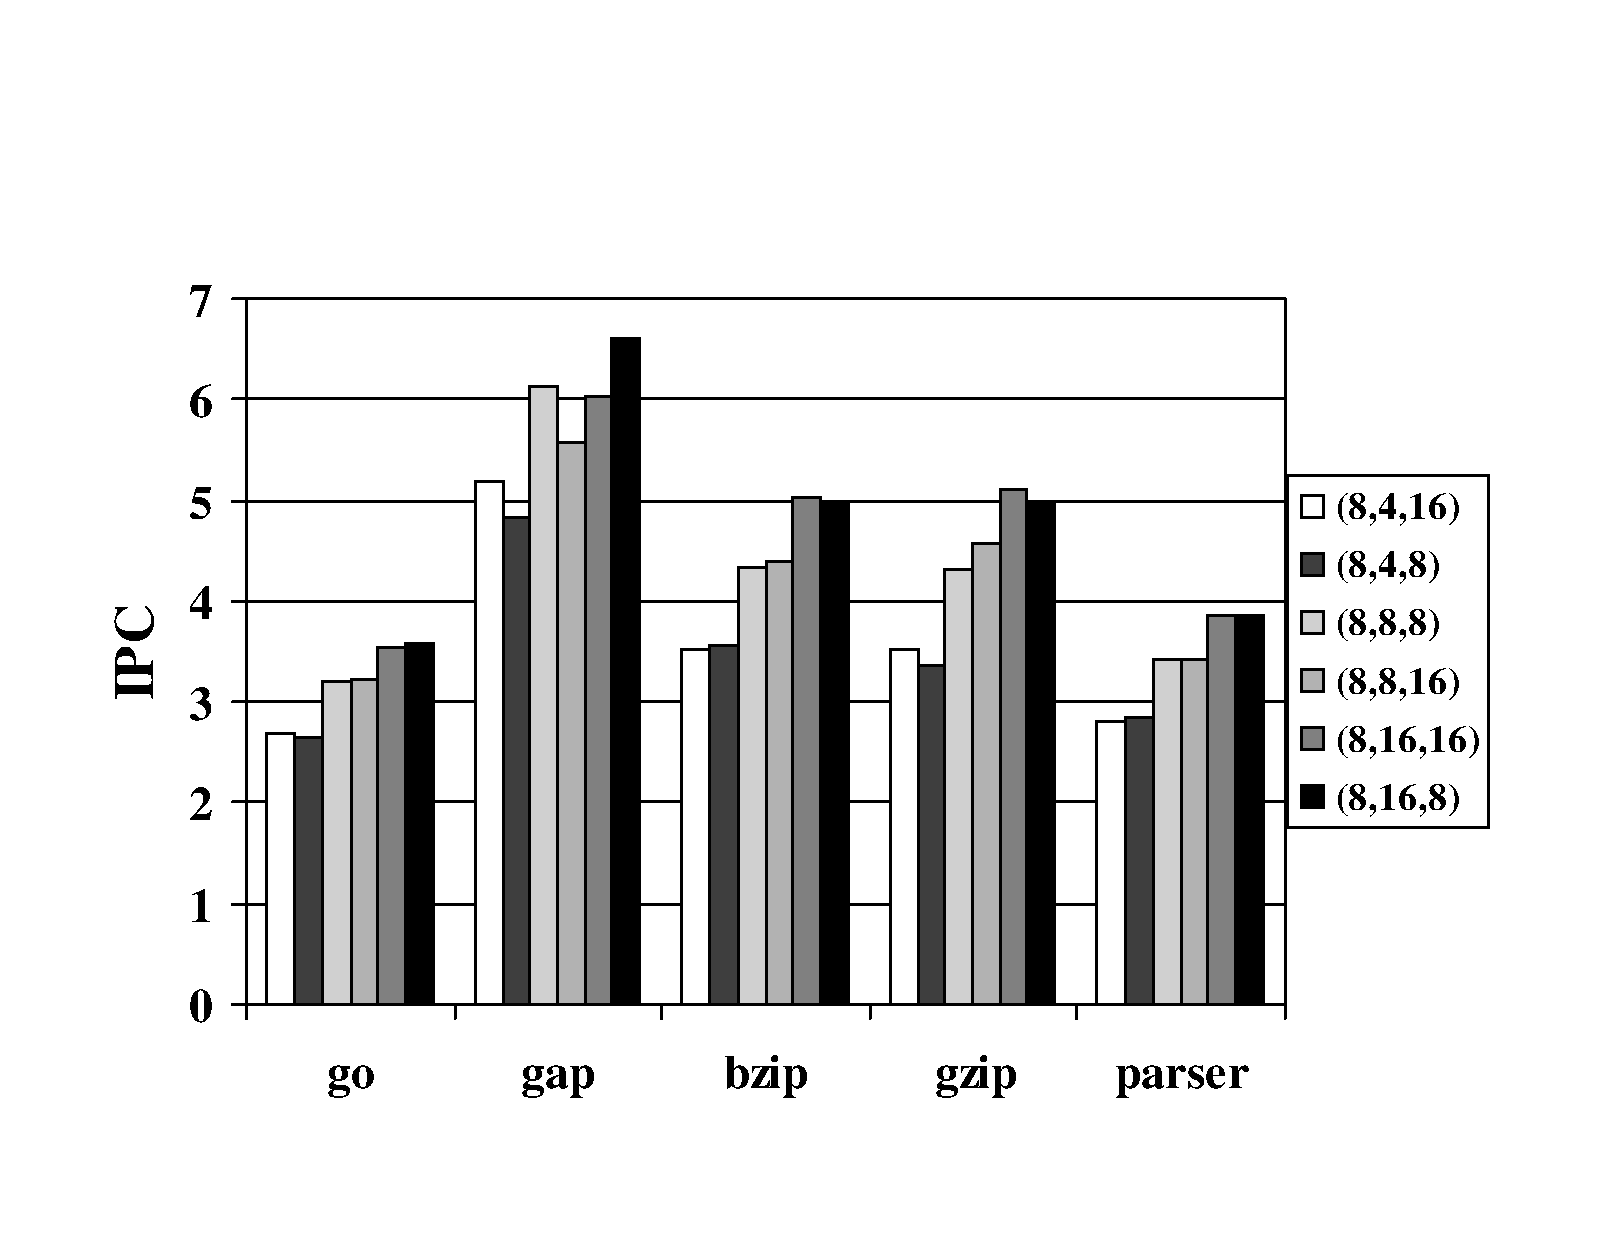
\epsfig{file=ics1.eps,width=5.8in}
\caption{{\em IPC Results for Varying Machine Configurations.} 
IPC results for several machine configurations is shown for each of
the five benchmark programs evaluated.}
\label{fig:ipc}
\end{figure}

Each of the machine configurations in Figure \ref{fig:ipc} consist of
three numbers that give the rows of sharing groups, the number of
active station rows per sharing group, and the number of sharing group
column respectively.  The number of sharing group rows times the number
of active stations per sharing group is the total number of active
stations rows in a configuration.  These are all issued instructions
together in a single clock.

As can be seen from the data, the configuration of 8-8-8 provides
the best overall IPC for the configurations simulated.  This consists
of 64 active stations in each column with 8 columns.
Configuration 16-8-4 does not perform as well because it does not
have as many columns (only 4 as compared with 8 in the other configuration)
to hide the latencies of instruction execution.  Eight columns 
hides more instruction execution latency than four.  The 8-4-16
configuration performs poorly as compared with 8-8-8 because the height
of a column (the primary IPC multiplier) is only 32 and its extra
columns are not needed to hide more instruction execution latency.
%
\subsection{Multipath Results and Discussion}
%
In this section we present data corresponding to varying the
maximum number of alternative speculative paths that are allowed.
Figure show the speedup results
when multipath execution is enabled.  Results for
each benchmark program is presented.  Results for each benchmark 
consists of six groups where each group represents the results
for one of six machine configurations.
The six machine configurations are :

\begin{tabular}{|c|c|c|c|}
\hline 
config&
SG rows&
ASes per SG&
SG columns\\
\hline
\hline 
1&
8&
4&
16\\
\hline 
2&
8&
4&
8\\
\hline 
3&
8&
8&
8\\
\hline 
4&
8&
8&
16\\
\hline 
5&
8&
16&
16\\
\hline 
6&
8&
16&
8\\
\hline
\end{tabular}

Speedups with each group of results is relative to the
Single Path (SP) case with no alternative speculative paths spawned
for any conditional branches.  For each benchmark program and
for each of the six machine configurations explored, speedups
for cases with a maximum
of zero (leftmost) to seven (rightmost) additional alternative 
paths are allowed.

\begin{figure}
\vspace{0.2 in}
\setlength{\epsfxsize}{14cm}%7
\centerline{\epsfbox{ics2.eps}}
%\centering
%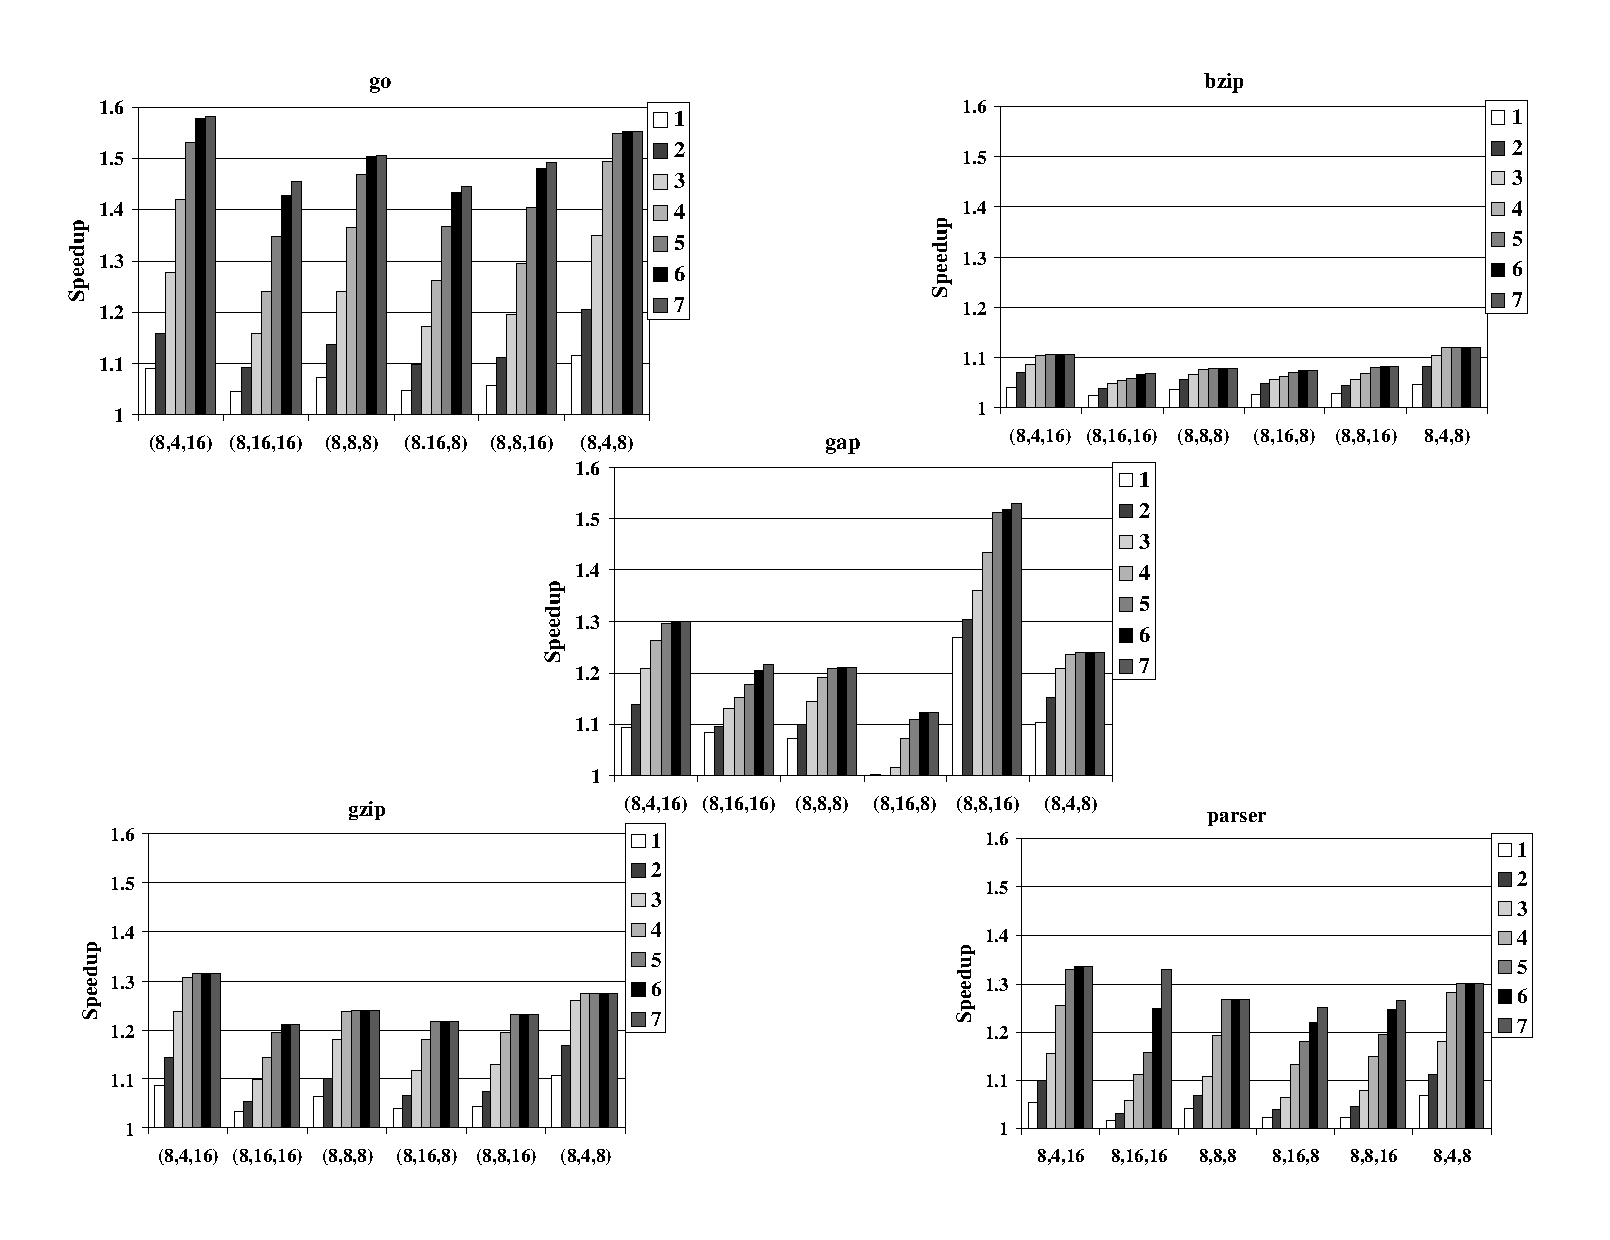
\epsfig{file=ics2.eps,width=6in}
\caption{ Multipath speedup for each benchmark.  $1-7$ denote the
spawning column. 
Speedups are relative to the Single Path (SP) execution case.}
\label{figall}
\end{figure}

%\begin{figure}
%\centering
%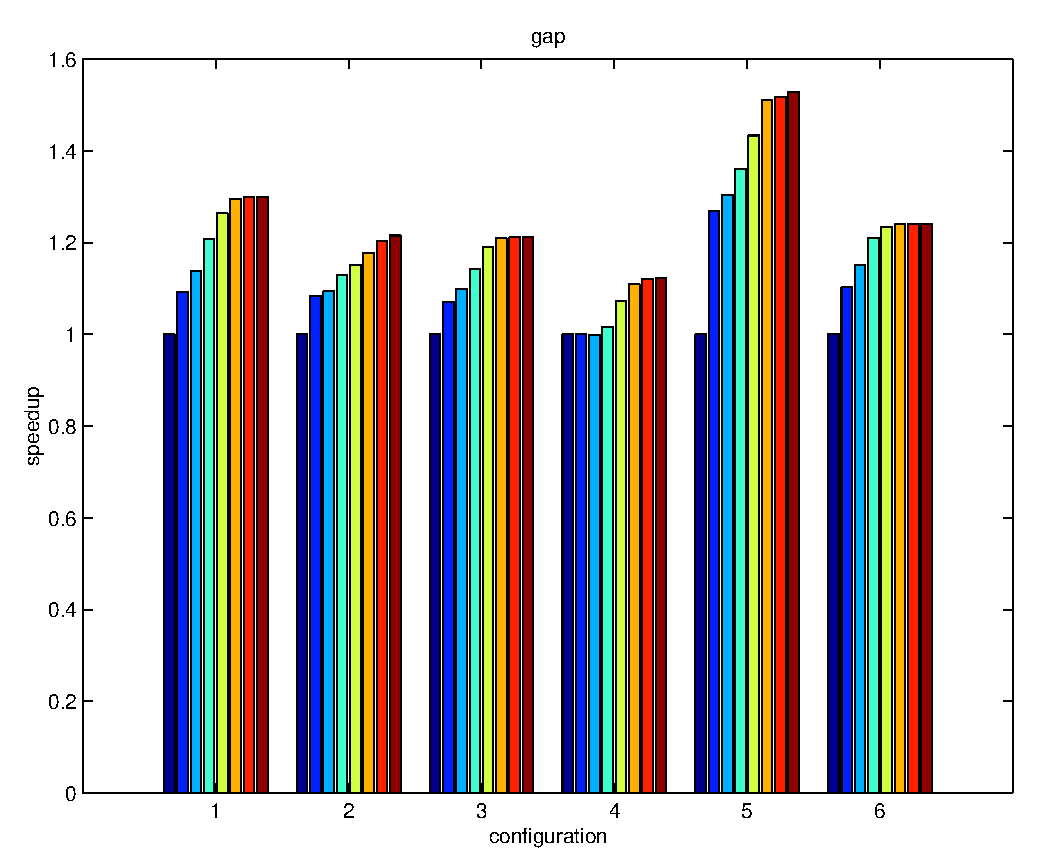
\epsfig{file=gap.eps,width=5.8in}
%\caption{{\em Multipath speedups for the BZIP2 benchmark program.} 
%IPC speedup results for several machine configurations is shown for 
%the GAP benchmark program.
%Speedups are relative to the Single Path (SP) execution case.}
%\label{fig:gap}
%\end{figure}

%\begin{figure}
%\centering
%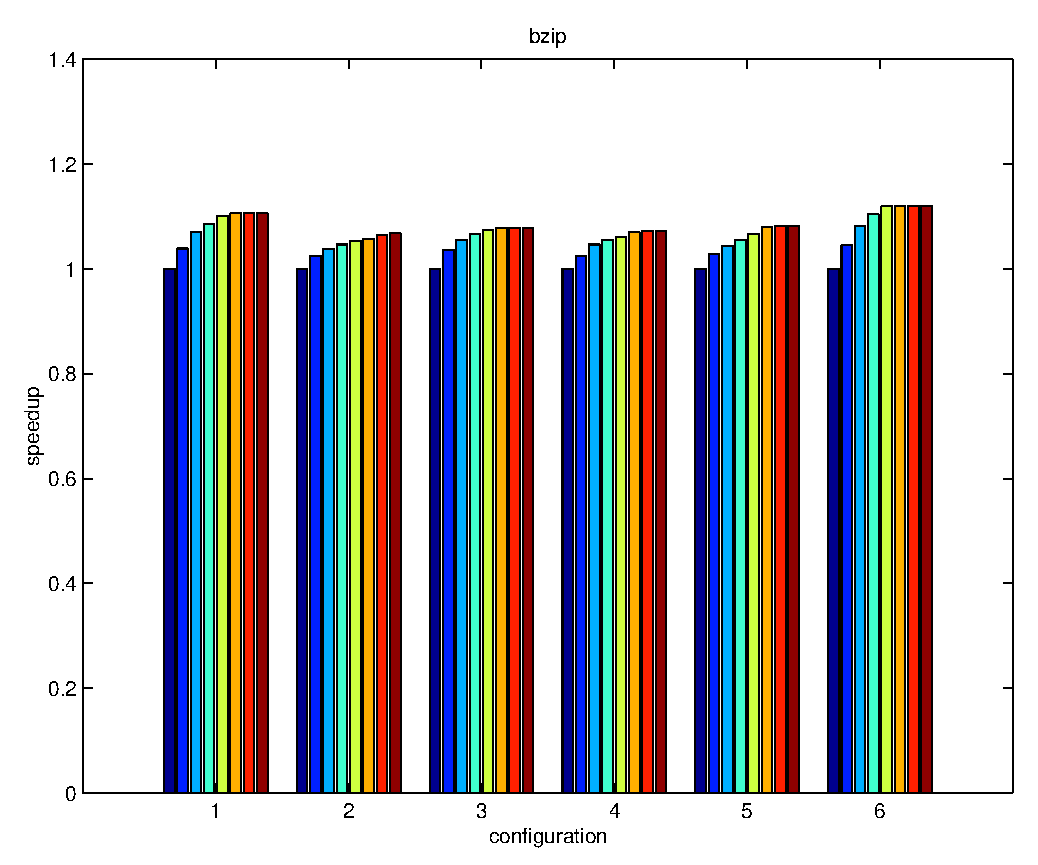
\epsfig{file=bzip2.eps,width=5.8in}
%\caption{{\em Multipath speedups for the BZIP2 benchmark program.} 
%IPC speedup results for several machine configurations is shown for 
%the BZIP2 benchmark program.
%Speedups are relative to the Single Path (SP) execution case.}
%\label{fig:bzip2}
%\end{figure}

%\begin{figure}
%\centering
%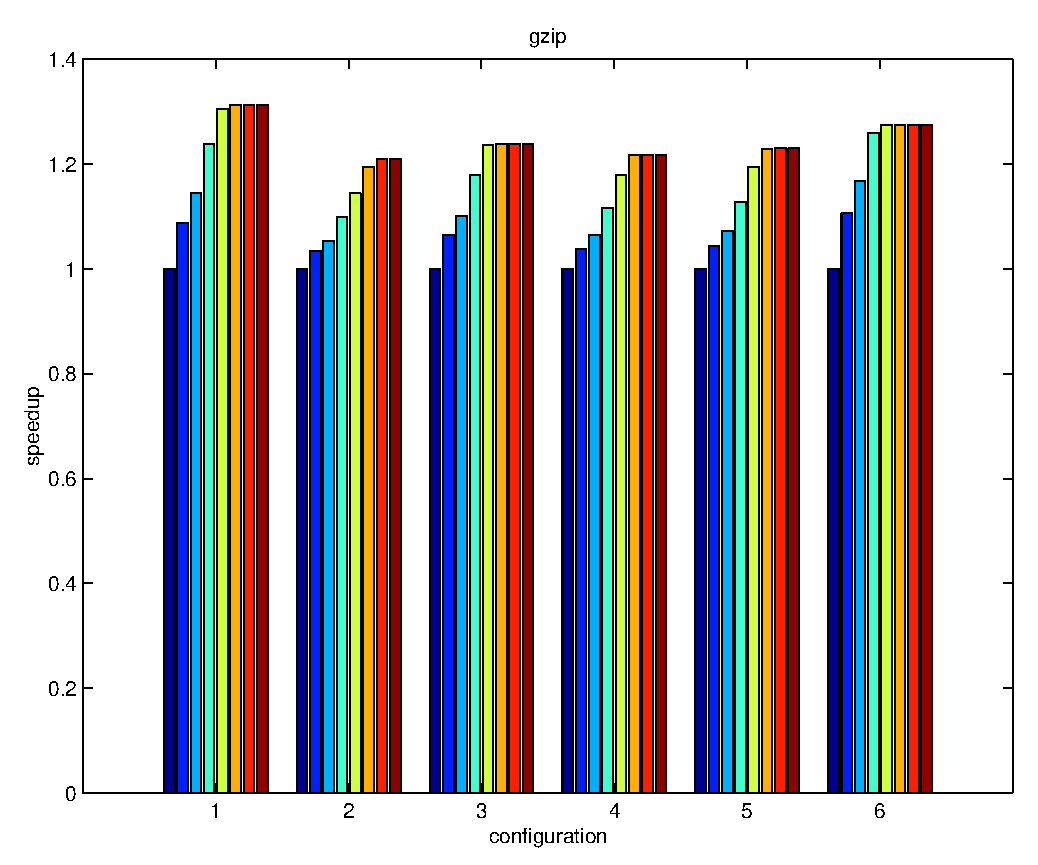
\epsfig{file=gzip.eps,width=5.8in}
%\caption{{\em Multipath speedups for the BZIP2 benchmark program.} 
%IPC speedup results for several machine configurations is shown for 
%the GZIP benchmark program.
%Speedups are relative to the Single Path (SP) execution case.}
%\label{fig:gzip}
%\end{figure}

%\begin{figure}
%\centering
%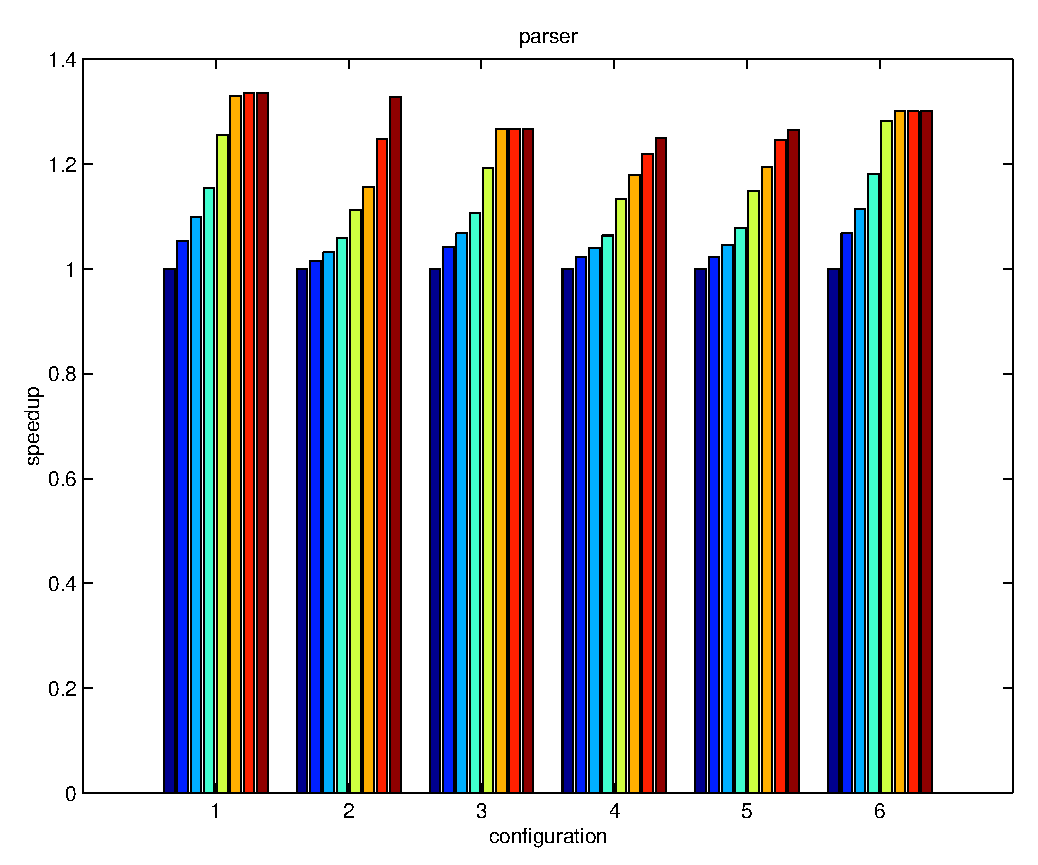
\epsfig{file=parser.eps,width=5.8in}
%\caption{{\em Multipath speedups for the BZIP2 benchmark program.} 
%IPC speedup results for several machine configurations is shown for 
%the the PARSER benchmark program.
%Speedups are relative to the Single Path (SP) execution case.}
%\label{fig:parser}
%\end{figure}

%
\section{Conclusions}
%
We have presented the overview of a large-scale distributed 
microarchitecture suitable for both extracting high ILP from
sequential programs and for implementing a scheme for
multipath execution.
Out simulation results have shown that .... !!!??


\bibliographystyle{latex8}
\bibliography{multi}

\end{document}
%
%
